\documentclass{article}
\usepackage[margin=1in]{geometry}
\usepackage{graphicx}
\usepackage{amsmath}
\usepackage{multirow}
\usepackage{multicol}
\usepackage{wrapfig}
\usepackage{algpseudocode}



%\topmargin 0pt
%\oddsidemargin 12pt
%\evensidemargin 12pt
\interfootnotelinepenalty=10000


\begin{document}
\title{Unsupervised Learning Segmentation of Objects in a Scene\\
\large  Project in COMP 652 and COMP 765}
\author{Yi Tian Xu\\260520039}

\maketitle

\abstract{}

%\begin{multicols}{2}

\section{Introduction}
Object manipulation and cognition are arguably a highly coupled task. For example, human infants can develop their manipulation skills through imitation \cite{cogn1}. For an autonomous robot, we thus image it to be driven by a continuous sequence of action, perception and reaction. In particular, it needs to identify and reason about its surrounding objects that potentially lie in a dynamic and unstructured environment. 

Recent studies in neural networks, in particular, Fully Convolutional Network (FCN) \cite{fcn} and Mask RNN \cite{rnn}, have risen as powerful tools in segmentation. Yet, as any supervised methods, a pre-defined labelled dataset provided by a human teacher may limit a robot in reasoning about novel objects. Moreover, robots who work in a specialized field, for example, pruning of city trees, would have supervised visual data that can be expensive to obtain, while robots with multi-dimensional specialities, for example a eldercare home robot, may require an extensive amount of data to cover all cases exhaustively.

In this work, we address to the problem of objects segmentation based on an unsupervised approach. We use motions to determine object boundaries and a probabilistic matching method to track the segments. In our setting, we will consider a passive robot that observes motions in its environment.

\section{Related Works}

\subsection{Segmentation Through Action}

Past studies have attempted to used robot's actions to coordinates its reasoning in detecting segments. For example, Hoof et al. \cite{herke} partitioned the environment into parts tracked by local key point descriptors, and developed a probabilistic model to infer the labelling of each part and to select best action to maximize information gain. As their approach rely on visual features detectable through Scale Invariant Feature Transform algorithm, the robustness to textureless objects is weak. Another disadvantage is that they ignore continuous observation of the objects and hand motion. Instead, they took snapshots of the scene before and after a robot action, and use Random Sample Consensus algorithm to find a rigid 3D transformation to track the parts. Due to a 1\% inaccuracy in their tracking algorithm due to, for example, illumination change and occlusion, the tracking error was accumulated action by action, and prevented the robot to correctly infer the number of segments in their experiment. 

Hoof et al. mentioned that their method is independent of the type of descriptor employed provided that the set of key points is sparse and each can be detected reliably from multiple views. Thus, expanding their method to low-texture object may simply require adding a new type of descriptors. However, we suggest that the use of continuous motion observation can provide enough information to track the parts without tracking key points. The main concern is to segment the hand from the object.

Correlation between the hand movement and the moved object may impose a challenge in discriminating the robot hand from touched object. Fitzpatrick et al. \cite{max-flow} experimented on segmenting one object of interest by making an impact movement on that object. They suggested to isolate the motion of the arm from the motion of the targeted object by comparing the image differencing before and after the moment of impact. We adopt their idea of using image differencing and attempt to expand their method to general hand-object movements and co-movement of objects.

\subsection{Gabor Filters}

As image differencing relies on the difference between pixel values in consecutive frames, it allows us to obtain a thin object boundary depending on the direction and the speed of the motion. Fitzpatrick et al. \cite{max-flow} used a maximum-flow algorithm for vision \cite{kolmo} to find the interior region of the object boundary. As am attempt for improvement, we will try to obtain a thicker object boundary allowing us to quickly fill the interior of the object. To this end, we refer to a well-known results in neuroscience to model the "eye" of the robot. 

Intuitively, if we trust that millions years of evolution has already provided us the optimized example of a vision system in ourself, why would one use a maximum-flow algorithm instead of a solution that is more biologically plausible?

employ gabor filters \cite{gabor} to magnify the edges. 

%% something about gabors and background substraction

\subsection{Image Region Tracking and Matching}

Object tracking based on points or descriptors, as in the work of Hoof et al. \cite{herke}, holds several challenges. Also discussed in the survey by Yilmaz et al. \cite{tracking}, such tracking requires some measurement of correspondence based on the motion of the tracked points or the entire object. Furthermore, the set of tacked key points often varies from frame to frame; old key poins may become occluded and new key points may emerge to light. Thus, a probabilistic approach represents a suitable solution to handle missing data and noisy observation. For multi-objects tracking, a clustering algorithm can be handy to distinguish between the object segments. 

In the context of multiple objects segmentation, reasoning in the movement correlation between tracked image regions may rise a concern in the trade-off between the number of regions tracked and the computational complexity. In Hoof et al.'s probabilistic method \cite{herke}, for example, tracked key points are initially partitioned into parts by a 3D grid covering the observed environment. Each part connects to a hidden markov model with known action and observed motion state, and latent segmentation labelling and true motion state. The computation of the probabilities growns exponentially as the number of parts increases. They therefore resort to Gibbs sampling to approximate the distribution. 

Shape matching represents an alternative approach to key points tracking \cite{tracking}. Shape, usually detected by background subtraction, can be complete object regions and large enough to overlap between frames. Matching is usually based on a similarity score with the hypothesized object model (e.g.: segmentation) generated by the previous frame. For example, Park et al. in their work for tracking and segmenting interacting human body parts \cite{human-action}, they employed many criteria to reason about image region similarity, namely color, border, size, orientation, neighbouring regions, etc. Others, mentioned by Yilmaz et al. \cite{tracking}, modelled shapes by color and edge histograms and used Bhattacharya distance or Kullback-Leibler divergence to establish similarity. Histogram is invariant to translation and rotation, and normalized histogram is invariant to scaling, providing convenience for representing shapes and evaluating similarities.

A motion-based approach to shape matching discussed by Yilmaz et al. \cite{tracking} is to evaluate the optical flow within the shape and use the dominant velocity vector to point to the corresponding shape in the next frame. This approach relies less on appearance invariance, which can be a solution to come of the crucial challenges in Park et al.'s image region matching problem.

Park et al. \cite{human-action} listed that a single shape can split to multiply shapes on the next frame and that multiple shape can merge into one shape on the next frame. In contrast to key points matching, shape matching is many-to-many and they can also appear and disappear from one frame to another. While Park et al. resolved their matching problem using multiple bipartite graph matching combined with hand turned heuristics, we attempt to use a combination of appearance-based and motion-based approach to track image regions and to match them to previously inferred segments. 

\subsection{Image Mutual Information}

Aside its application in tracking, mutual Information (MI) has been a common measurement tool for image comparison in clinical applications \cite{mi}, in particular for aligning 2D images to form 3D images. At the heart of the technique is the designation of the marginal and joint histogram as the image distribution. In this formulation, each pixel is a random variable. The marginal histogram counts the occurrence of pixel values in the image, while the joint histogram counts the co-occurrence of pixel pair values in two image, which is a 2D histogram. 

Marginal and joint histograms are then used to compute marginal and joint entropy, which are subsequently used to compute MI. Maximizing MI over images transformation (e.g.: rotations and translations) approximates the best alignment. This assumes a statistical relationship between two images which can be captured by the joint entropy. Maximizing MI is thus related to minimizing the joint entropy. Yet, the joint entropy may encounter some edge case problem when used alone, as argued by Pluim et al. \cite{mi}. (?)

The independence of visual features and the lack of parameter tuning have given mutual information success in the medical domain. Pluim et al. showed in their survey a diversity of variation of MI, including normalized MI and MI that includes spacial information by consider one neighbouring pixel value. Russakoff et al. \cite{rmi} proposed regional mutual information, extending the idea of spacial information inclusion by considering all neighbouring pixel valus in a $nxn$ neighbourhood, creating $n\times n$-dimensional marginal histograms and $2n\times n$-dimensional joint histograms. Computational complexity can be optimized using PCA and the performance is asymptotically close to the original MI as the neighbourhood radius is fixed. 

Although Russakoff et al. showed that RMI is more robust to noise than the original formulation of MI and the variations explored by Pluim et al, we will use the original formulation of MI as a measure to match segments between frames and to experiment its performance in our problem context. 

\section{Method}

\begin{figure}[tbp]
\begin{center}
\caption{Visualization of the method: (A) Input frame is being processed to (B, C, D and E). (B) Background average is accumulated with the new frame. (c) Image difference detects movement. (D) Gabor filtering detects edges in the current frame (also on the background (B), not shown in image). (E) Image differencing between gabor filtered background and (D) results image parts that can be mapped to segments. (F) Finally, a probabilistic matching method infer the labellings of the parts in (E) according to the previously inferred segments.}
  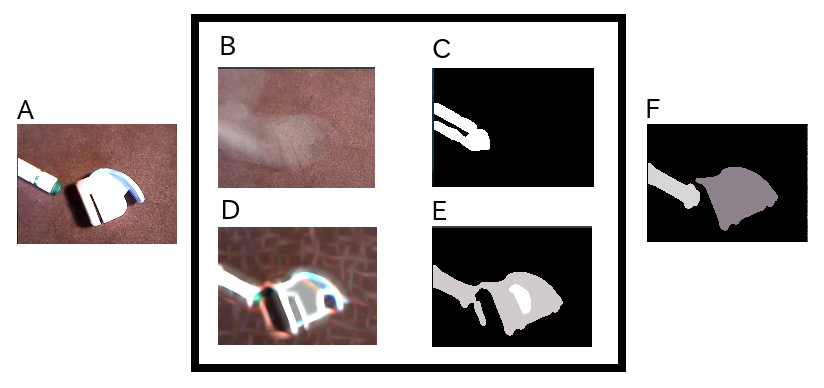
\includegraphics[width=0.9\textwidth]{1}
\label{figure:model_seq}
\end{center}
\end{figure}

\subsection{Filtering and Part Extraction}

To allow the gabor filter running close to real-time, we had to downside the image to 160 $\times$ 120 px. 

At each frame, we add it to the background average and we use image differencing to detect motion. When a considerably large motion is detected, we preform gabor filtering on the background average and the most recent frame. In our experiment, we used $n_g=$ 55 differently oriented gabors of $s_g=$ 12 px in size. Only cosine gabors are considered although integration of sine gabors is possible. (and inversed cosine gabors) A second image differencing between the two filtered images, which is equivalent to a background subtraction, yields isolation of moved edges. 

To obtain a clean image of the moved edges, we had to add a few other filters before and after the gabor filters, namely Gaussian blur and thresholding. Below is the pseudocode for parts extraction.\\

\begin{algorithmic}[H]
	\Function{PartsExtraction}{RGB image frame $I$, RGB background average $B$}
		\State $I' \leftarrow$ GaborFilter($I$)
		\State $B' \leftarrow$ GaborFilter($B$)
		\State $P \leftarrow$ AbsoluteDifference($I'$, $B'$)
		\State $P \leftarrow$ GaussianBlur($P$, $\sigma$)
		\State $P \leftarrow$ Thresholding($P$, $\theta_1$)
		\State $P \leftarrow$ SplitIntoContours($P$, MIN\_COUNTOUR)
		\State \Return $P$
	\EndFunction 
\end{algorithmic}

\begin{algorithmic}[H]
	\Function{GaborFilter}{Image $I$}
		\State $I_1 \leftarrow$ GaussianBlur($I$, $\sigma$)
		\State $I_2 \leftarrow I_1$
		\For{each gabor kernel $k$}
			\State $I_2 \leftarrow \max$(Convolution($I_1$, $k$), $I_2$)
		\EndFor
		\State $I_2 \leftarrow$ Thresholding($I_2$, $\theta_2$)
		\State \Return $I_2$
	\EndFunction
	
\end{algorithmic}

The Gaussian blur preforms a Gaussian averaging for each pixel with a neighbouring spread of $\sigma$. The thresholding segments the image into two parts with the cutoff pixel value $\theta_i$. The parameter $\sigma$ is tuned to 11 in the experiment. $\theta_1$ and $\theta_2$ are set to be the standard deviation of the pixel values for the gabor filtered frame image and the mean increased by $t$ times of the standard deviation of the gabor filtered frame image respectively. $t$ is set to 1.7 in the experiment. 

The size of the Gaussian blur ($\sigma$) affects the performance of the gabor filters. We added blurring prior to the gabor filter to soften the shadow and to smooth the extracted edges (see Figure \ref{figure:gaussian_blur}). A additional Gaussian blur is used after the gabor filter accompanied with thresholding to smooth further the edges and to remove noise. 

\begin{figure}[tbp]
\begin{center}
\caption{Comparison between non-blurring(B, C) and blurring (D, E) prior to gabor filtering. (A) The original scene frame.  (D) Detected edges without Gaussian blur prior to gabor filtering, and (C) with Gaussian blur and thresholding after gabor filtering. (D) Detected edges with Gaussian blur prior to gabor filtering, and (E) finalized with another Gaussian blur and thresholding.}
  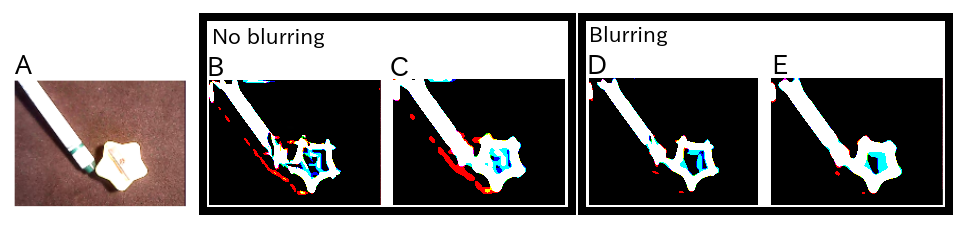
\includegraphics[width=0.95\textwidth]{2}
\label{figure:gaussian_blur}
\end{center}
\end{figure}


The last operation in the parts extraction function, \emph{SplitIntoContours}, finds the contours and fill-in colors. This is a quick heuristic to segment moved object from the background, assuming that all objects with no visible holes (topology (?)...). The obtained segmentation is used a partitioning of the image that shall feed the probabilistic matching method to infer and track the final object segments. 

\subsection{Probabilistic Matching}

Scoring similarity may not necessitate a probabilistic approach as simply maximizing a similarity scores can be enough to find the best matching. However, since the set of elements to match changes from frame to frame, modelling each inferred segment as a normalized weight vector of labellings may be more intuitive in three ways: (1) ambiguous image regions can be resolved after observing more evidence(s) (2) uncertainly in the appearance or disappearance of a segment can also be capture in the probabilistic model, and (3) normalization enables comparison of scores between different elements. 

\subsubsection{Similarity Measure}

Both the motion detected through image differencing (which we will call motion image henceforth) and the image with the extracted parts are considered in our probabilistic matching model. Let $R_t$ be a part extracted at time $t$ and $M_t$, the motion image computed at the same time. We compute the probability of $R_t$ being labelled by $l$ given motion image as
\begin{equation}
	P(R_t = l | M_t) = \sum_{S_{t-1}} P(R_t = S_{t-1} | S_{t-1}, M_t)P(S_{t-1} = l)
\end{equation}
where $S_{t-1}$ is the segments inferred from the previous time step. $P(R_t = S_{t-1} | S_{t-1}, M_t)$ is estimated using MI between the newly extracted part, the previous inferred segment and the motion image. We assume that 
\begin{equation}\label{eq:blab}
	P(R_t = S_{t-1} | S_{t-1}, M_t) \propto F_{MI}(R_t; S_{t-1})D(F_{MI}(R_t; M_t) + \epsilon, F_{MI}(S_{t-1}; M_t) + \epsilon)
\end{equation}
where
\begin{equation}
	F_{MI}(A;B) = \frac{MI(A;B)}{H(A)}
\end{equation}
where $MI$ is the image mutual information and $H$ is the entropy functions. We found that $F_{MI}$ is a more suitable score to establish similarity in this context. As MI is not upper bounded, reasoning in whether a MI score is large enough to determine a matching as opposed to no matching at all is not well-defined. Different from the medical application where a true image alignment is usually guaranteed to exists, our context often encounters the case when the extracted part $R_t$ is truly a new segment. In such case, maximizing MI between previously inferred segments will inevitably give the wrong solution. We therefore normalize MI with the extracted part's entropy to upper bound the score by 1. The score is exactly 1 when the compared images are identical. 

Equation \ref{eq:blab} thus conducts three comparisons. The similarities between $R_t$ and $M_t$, and $S_{t-1}$ and $M_t$ are combined and reweighed by the function $D$. Intuitively, image parts and inferred segments are probabilistically more likely to match if they are both matching the motion image, or both not matching the motion image. In other words, the matching should be consistent with the observed motion. Thus, we choose
\begin{equation}
	D(A,B) = -\log\left(1-\min\left(\frac{A}{B}, \frac{B}{A}\right)\right)
\end{equation}
The choice of using the minimum ratio between $A$ and $B$ is to bound the range of $D$ between $0$ and $\infty$. The negative logarithm function will allow $D$ to increase rapidly as $A$ and $B$ becomes closer in value. Since the function is undefined when $A$ or $B$ equals to 0, we add a small value, $\epsilon$, in Equation \ref{eq:blab} to ensure that the input is never 0. In the context of Equation \ref{eq:blab}, $D$ will reach maximum value only if comparisons of the regions $R_t$ and $S_{t-1}$ with the motion $M_t$ yield identical $F_{MI}$ values. $D$ will tend to 0 when the $F_{MI}$ values are largely different. As $F_{MI}$ is designed to measure image similarity, $D$ is designed to measure similarity of similarities.

We have also consider other function choices for $D$. For example, we can also choose to have $D$ increase linearly or in a polynomial fashion. The percentage difference, the Euclidean distance, standard deviation, etc, can also shape the design for $D$. However, results from our experiment showed that a rapidly growing $D$ is more suitable. We will discuss further on the choice of $D$ in Section \ref{sec:exp}.

\subsubsection{Appeared and Disappeared Image Regions}

Park et al. mentioned that object segments can appear and disappear due to occlusion, shadowing and overlaps \cite{human-action}. To address to this issue, we introduce a segment decay parameter $\alpha$, which we set to 0.05 in our experiment. At each time step, each inferred segment will have all their label probability reduced by $\alpha$ (i.e.: $P(S_{t} = l)$ for every segment $S_t$ and labelling $l$ is updated to $(1-\alpha)P(S_{t} = l)$ at the end of each iteration). If the segment is no longer matched to any newly observed image part(s), it will keep decaying and will eventually vanish. Otherwise, we replace its labelling probabilities with ones of the matched image part(s). 

The decay factor applied onto the labelling probabilities after $\tau$ consecutive times steps with no matching is $(1-\alpha)^{\tau}$, implying a probability of $1- (1-\alpha)^{\tau}$ that the decaying segment should be assigned to a new labelling. We do not use this implication directly to decide whether a new labelling should appear. Instead, we called this probability the "decay weight" of a segment ($d_{S_t}$) and use the average of the decay weights over all inferred segments rescaled by the variance of the comparison scores for each image part to decide whether that part should be assigned to a new labelling. 

The reason for using the variance (or standard deviation) in the decision of adding new labelling refers to the idea that an image part that equally similar to all previously inferred segments should either matches all those segments or none of them depending on how similar it is to all those segments. As explained in the previous section, it is for this reason that an upper bounded similarity score becomes crucial in this matching problem and our $F_{MI}$ function can provide the need. 

In summary, the probability for part $R_t$ to be aligned to a new label $l'$ is 
\begin{equation}
	P(R_t = l' | M_t) \propto \left(\frac{1}{n_{t-1}} \sum_{S_{t-1}}(d_{S_{t-1}})\right)\mathcal{S}(R_t, M_t, C)
\end{equation}
where $n_{t-1}$ is the number of inferred segment at time step $t-1$ and $\mathcal{S}(R_t, M_t, C)$ is the standard deviation of the similarities scores as computed by Equation \ref{eq:blab} over all inferred labelling scaled by some constant $C$. In our experiment, we choose to multiply the standard deviation by $c = 100$. In the case when there is only one inferred segment, we set $\mathcal{S}(R_t, M_t, C) = 1$. 

\subsubsection{Merging and Splitting Image Regions}

Park et al. also mentioned that previously inferred segments can split or merge into others also due to similar optic effects \cite{human-action}. Furthermore, we do no employ any particular algorithm to optimize the matching time. As a brute force search is used, the number of comparisons grows exponentially in the number of elements to compare. Hence, merging parts that are most likely matched to the same labelling presents an option that benefit the computational complexity. 

Let $\pi_{P_i}$ be the vector of probabilities for part $P_i$. Suppose that label $l$ has maximum probability for all $P_i$ for $i\in \{1,...,k\}$, i.e.: $\max_j \pi_{P_i}[j] = \pi_{P_i}[l],  \forall i\in \{1,...,k\}$. After merging, we recompute the probability of the merged part for each labelling, obtaining merged part $P'$ and probability vector $\pi_P$. We can further compare $\pi_P[l]$ with the $\pi_{P_i}[l]$, perhaps by assessing whether $\pi_P[l] > E[\pi_{P_i}[l]]$ or $\pi_P[l] > \max_i (\pi_{P_i}[l])$. This may give a better measure for keeping the merging or not. However, we decided to not conduct any of such evaluation.

\section{Experiment}\label{sec:exp}

% filtering cut theta and sigma with number of gabor and size 
% decay param 

\section{Discussion}

Use binary search to first to see which region in a larger scene a moved object can be matched to.

Allow robot to grab object and observe the patterns and shapes which can be learn with a FCN. Allow communication between human teacher and a robot where teacher points and name the object and robot can go grab that object and learn it.  

Perhaps add feature tracking for occluded objects. 

\section{Conclusion}


\begin{thebibliography}{9}

\bibitem{cogn1}
	A. N. Meltzoff
	\emph{Infant Imitation After a 1-Week Delay: Long-Term Memory for Novel Acts and Multiple Stimuli.}
	Developmental Psychology (1988) Vol 24, No 4, 470-476.
	
\bibitem{fcn}
	J. Long, E. Shelhamer, and T. Darrell. 
	\emph{Fully convolutionalnetworks for semantic segmentation.}
	CVPR, 2015

\bibitem{rnn}
	K. He, G. Gkioxari, P. Doll\`ar, R. Girshick
	\emph{Mask R-CNN.}
	
\bibitem{herke}
  H. V. Hoof, O. Kroemer, and J. Peters
  \emph{Probabilistic Segmentation and Targeted Exploration of Objects in Cluttered Environment.}
  
\bibitem{max-flow}
	P. Fitzpatrick and G. Metta 
	\emph{Grounding Vision Through Experimental Manipulation.}
	Philos. T. Roy. Soc. A (2003) Vol. 361, No. 1811, 2165-2185
	
\bibitem{kolmo}
	Y. Boykov and V. Kolmogorov
	\emph{An Experimental Comparison of Min-Cut/Max-Flow Algorithm for Energy Minimization in Vision.}
	Energy Minimization Methods in Computer Vision and Pattern Recognition (2001) 359-374

\bibitem{gabor}
	R. Mehrotra
	\emph{Gabor Filter-Based Edge Detection.}
	
\bibitem{tracking}
	A. Yilmaz
	\emph{Object Tracking: A Survey} ACM Computing Surveys, Vol. 38, No. 4, Article 13, Publication date: December 2006.

\bibitem{human-action}
	S. Park and J. K. Aggarwal
	\emph{Segmentation and Tracking of Interacting Human Body Parts Under Occlusion and Shadowing.} Workshop on Motion and Video Computing, Orlando, Florida (2002), 105-111

\bibitem{mi}
	J. P. W. Pluim
	\emph{Mutual Information based Registration of Medical Images: a Survey.}
	
\bibitem{rmi}
	D. B. Russakoff
	\emph{Image Similarity Using Mutual Information of Regions.}
	
\end{thebibliography}
%\end{multicols}
\end{document}